\section{A worked three-mass example}\label{sec:spring}
The chain makes the construction explicit: fit the endpoint transfer,
complete one missing row, and predict the middle response.
\begin{figure}[tbp]\centering
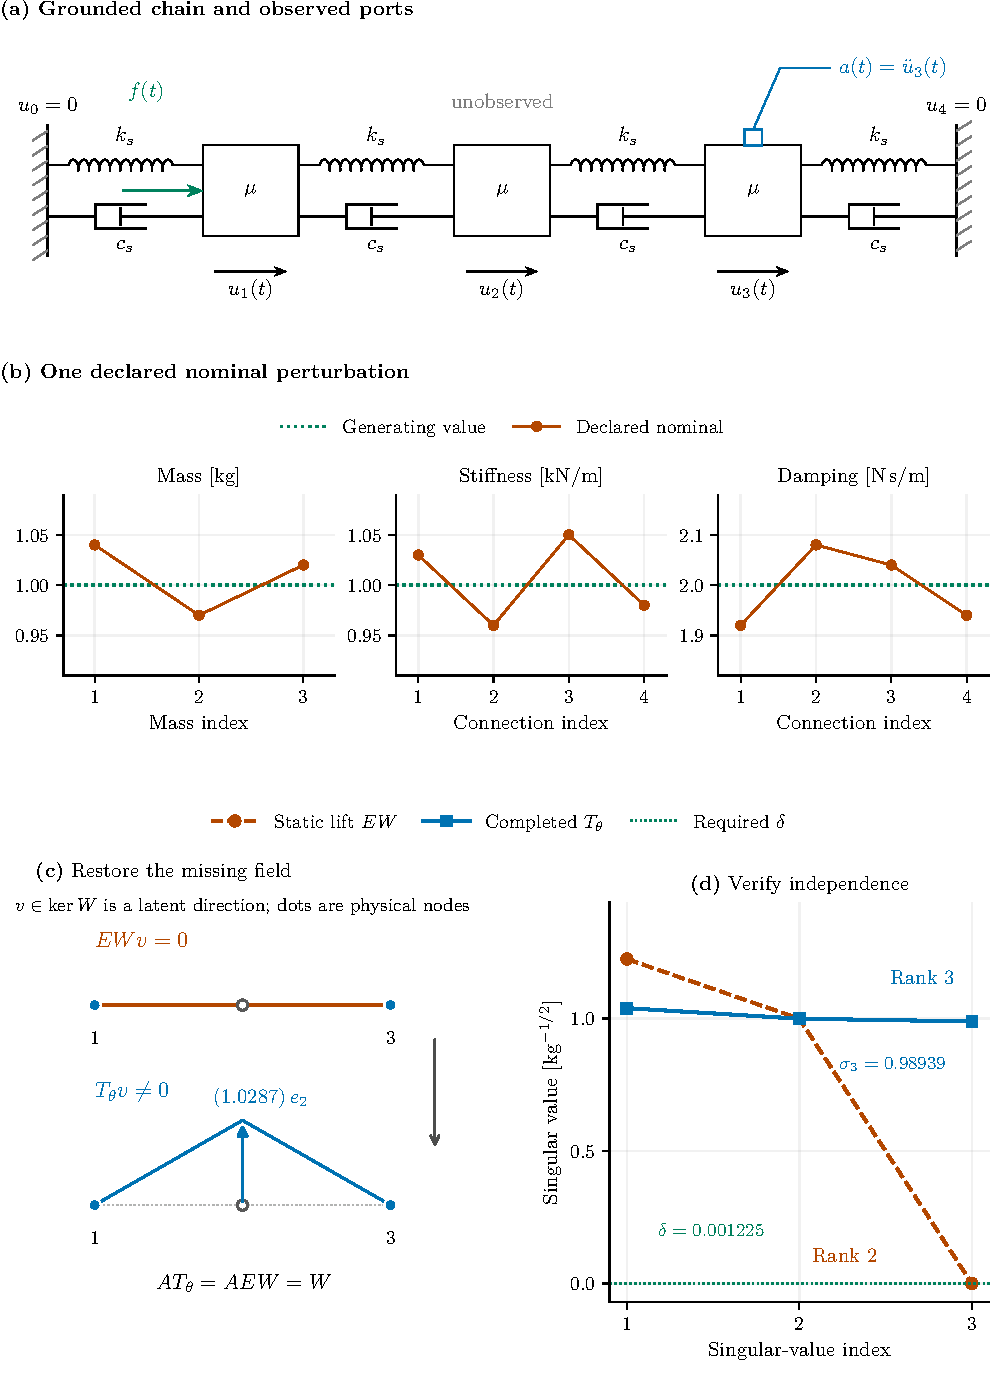
\includegraphics[width=\linewidth]{spring_overview.pdf}
\caption{Three-mass construction. (a) Force at mass 1, acceleration measured at
mass 3. (b) Nominal and generating parameters. (c) A unit $v\in\ker W$
gives $EWv=0$ but $T_\theta v\ne0$: completion supplies the missing middle
motion, in kg$^{-1/2}$. (d) Rank increases from two to three.}
\label{fig:spring-overview}
\end{figure}

\subsection{Fit the endpoint transfer}
Let $e_i$ denote physical coordinate $i$ and let the chain incidence matrix
$D_{\rm c}$ have rows $(1,0,0)$, $(-1,1,0)$, $(0,-1,1)$ and $(0,0,-1)$.
The generating system, used only for observations and assessment, is
\begin{equation}
 M_*=I_3\ \mathrm{kg},\qquad
 C_*=2D_{\rm c}^{\top}D_{\rm c}\ \mathrm{N\,s/m},\qquad
 K_*=1000D_{\rm c}^{\top}D_{\rm c}\ \mathrm{N/m}.
 \label{eq:spring-matrices}
\end{equation}
Only the endpoint transfer $a_3/f_1$ is fitted. Thus $n=r=3$, $h=2$,
$p=m=1$, and
\begin{equation}
 B=e_1,\quad S=e_3^{\top},\quad
 A=\begin{bmatrix}e_1^{\top}\\e_3^{\top}\end{bmatrix},\quad
 W=AT=\begin{bmatrix}T_{1,:}\\T_{3,:}\end{bmatrix},\quad
 R_{\rm i}=[1,0],\quad R_{\rm o}=[0,1].
 \label{eq:spring-registration}
\end{equation}
The middle row $T_{2,:}$ does not enter the fitted transfer.

There are 2381 complex samples on 0.1--12 Hz at 0.005 Hz spacing.
Independent real and imaginary Gaussian noise has total complex variance
$0.02^2(\rho_*^2+|H_{31,*}(\nu)|^2)/2$, where $\rho_*$ is the generating
transfer's band RMS. Training and assessment seeds are 20261031 and 20261101.
The fit uses $b=2$, $\alpha=10^{-5}$ and the first-difference penalty
$G=\left[\begin{smallmatrix}3/4&-1/4\\-1/4&3/4\end{smallmatrix}\right]$, normalized as in Appendix~\ref{sec:fit-details}.
Its fitted parameter is
\begin{equation}
 \begin{aligned}
 W&\simeq\SpringW\ \mathrm{kg}^{-1/2},\\
 \Omega^{2}&\simeq\diag(\SpringOmegaSquared)\ \mathrm{s}^{-2},\\
 \Gamma&\simeq\SpringGamma\ \mathrm{s}^{-1}.
 \end{aligned}
 \label{eq:spring-factors}
\end{equation}
The undamped frequencies are 3.851863, 7.117600 and 9.298528 Hz;
the quadratic pencil has three conjugate pole pairs. Frequencies order the
columns, the largest entry fixes each column's sign, and the penalty fixes
the reciprocal scale. Calculations retain full precision, including entries
rounded to zero above. Training and independent noisy errors are
\SpringTrainingError\% and \SpringIndependentError\% on the training scale
$d_{31}$; these do not establish uniqueness of $\theta$.

\subsection{Complete the missing row}
The fixed prior uses $(m_1,m_2,m_3)=(1.04,0.97,1.02)$ kg and
$(k_1,k_2,k_3,k_4)=(1030,960,1050,980)$ N/m:
\begin{equation}
 M_0=\diag(m_1,m_2,m_3),\qquad
 K_0=\begin{bmatrix}
 k_1+k_2&-k_2&0\\-k_2&k_2+k_3&-k_3\\0&-k_3&k_3+k_4
 \end{bmatrix}.
 \label{eq:spring-prior}
\end{equation}
The baseline curve also uses
$C_0=D_{\rm c}^{\top}\diag(1.92,2.08,2.04,1.94)D_{\rm c}$ N\,s/m.
Only $M_0,K_0$ enter completion. The middle response selects none of these
parameters.

The constraint $AT=W$ fixes the end rows of $T$, so only the middle row is
free. We write it as the static interpolation of the end rows plus a
correction. For prescribed endpoints, minimum elastic energy gives
\begin{equation}
 \bar u_2=\argmin_{u_2}
 \left\{\tfrac12k_2(u_2-u_1)^2+\tfrac12k_3(u_3-u_2)^2\right\}
 =\frac{k_2u_1+k_3u_3}{k_2+k_3}.
 \label{eq:spring-elastic-square}
\end{equation}
The static lift and the only port-invisible direction are therefore
\begin{equation}
 E=\begin{bmatrix}1&0\\32/67&35/67\\0&1\end{bmatrix},\qquad
 N=\frac{e_2}{\sqrt{m_2}},\qquad AE=I_2,\quad AN=0,
 \label{eq:spring-lift}
\end{equation}
and every member of $\mathcal T(\theta)$ has the form
\begin{equation}
 T=EW+NZ=\begin{bmatrix}
 W_{1,:}\\ (32W_{1,:}+35W_{2,:})/67+Z/\sqrt{m_2}\\W_{2,:}
 \end{bmatrix},\qquad Z\in\R^{1\times3}.
 \label{eq:spring-T}
\end{equation}
There is one hidden spatial direction $e_2$ but three modal columns, so
$Z=[z_1,z_2,z_3]$ has one entry per mode. The static map $EW$ has rank two.

The chain data are synthetic FRFs without a force record, so
Eq.~\eqref{eq:Pi} uses a unit force spectrum on the fitted grid:
\[
 \Phi_q\simeq10^{-6}\SpringPi\ \mathrm{kg\,m^2}.
\]
The modes are almost uncorrelated; the largest correlation is
\SpringPiCorrelation. With $c_j=(K_0-\omega_j^2M_0)N$ and
$a_j=(K_0-\omega_j^2M_0)Ew_j$, column $j$ of $G$ is $a_j+c_jz_j$, so $J_F$
is a quadratic in $Z$ with minimizer
\begin{equation}
 Z^{\top}=-\mathcal H^{-1}b,\qquad
 \mathcal H_{jk}=(\Phi_q)_{jk}\,c_j^{\top}K_0^{-1}c_k,\qquad
 b_j=\sum_k(\Phi_q)_{jk}\,c_j^{\top}K_0^{-1}a_k.
 \label{eq:spring-scalar}
\end{equation}
Numerically $\mathcal H\simeq10^{-3}\SpringH$ and
$b^{\top}\simeq10^{-3}\Springb$, which give
\begin{equation}
 Z\simeq\SpringZ,\qquad
 T_\theta\simeq\SpringT\ \mathrm{kg}^{-1/2}.
 \label{eq:spring-completed}
\end{equation}
Nearly equal endpoint patterns $w_1,w_3\simeq(0.5,0.5)^{\top}$ receive
opposite middle entries $\SpringHiddenFirst$ and $\SpringHiddenThird$. Their
frequencies of 3.85 and 9.30 Hz enter through $c_1$ and $c_3$. Because the
modes are nearly uncorrelated, $T_\theta$ differs from the undamped
per-mode solution by only \SpringMapChange\%.

The margin is $\delta=10^{-3}\sigma_1(EW)=\SpringMargin$ kg$^{-1/2}$. The
equality-only map already meets it, with
$\sigma_3(T_\theta)=\SpringSigmaMin$ kg$^{-1/2}$ and
$\kappa_2(T_\theta)=\SpringCondition$. By
Theorem~\ref{thm:completion}(iii) it solves
Eq.~\eqref{eq:completion-problem}, and no iteration is needed. The
criterion falls from $J_F(\theta,EW)=\SpringJFStatic$ to
$J_F(\theta,T_\theta)=\SpringJF$, and $\|VT_\theta-I_3\|_F=\SpringLeftInverse$.
For $v\in\ker W\setminus\{0\}$, $EWv=0$ but $T_\theta v=NZv\ne0$: the
missing direction survives without moving either port.

\subsection{Preserve the endpoint response, predict the middle}
The payoff is visible directly in the two transfers:
\begin{align}
 H_{31}(s)&=s^2W_{2,:}\Delta_\theta(s)^{-1}W_{1,:}^{\top},\nonumber\\
 H_{21}(s)&=s^2\underbrace{\left(
 \frac{32W_{1,:}+35W_{2,:}}{67}+\frac{Z}{\sqrt{m_2}}\right)}_{T_{\theta,2,:}}
 \Delta_\theta(s)^{-1}W_{1,:}^{\top}.
 \label{eq:spring-transfers}
\end{align}
Only the middle response depends on $Z$. Since $n=r=3$, $T_\theta$ is
invertible and the displacement-coordinate matrices are
\begin{align}
 M_\theta=T_\theta^{-\top}T_\theta^{-1}&\simeq\SpringM\ \mathrm{kg},\label{eq:spring-mck}\\
 C_\theta=T_\theta^{-\top}\Gamma T_\theta^{-1}&\simeq\SpringC\ \mathrm{N\,s/m},\label{eq:spring-c}\\
 K_\theta=T_\theta^{-\top}\Omega^2T_\theta^{-1}&\simeq\SpringK\ \mathrm{N/m}.\label{eq:spring-k}
\end{align}
Latent and physical accelerances agree to \SpringPhysicalResidual\ relative
error. State-space displacement, velocity and acceleration checks also agree.

\begin{figure}[tbp]\centering
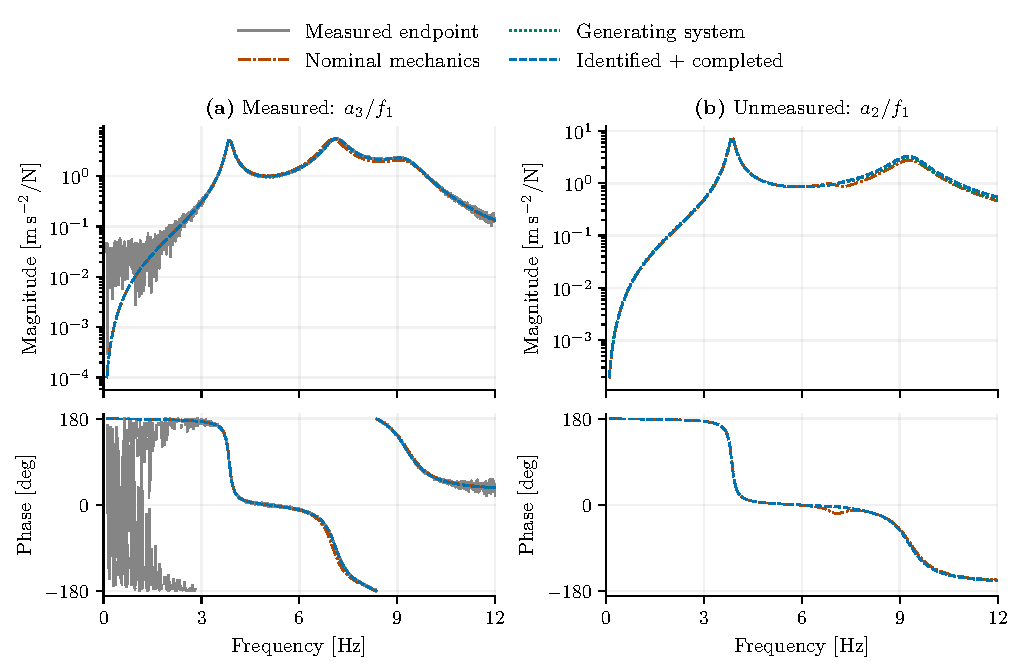
\includegraphics[width=\linewidth]{spring_frf.pdf}
\caption{Chain accelerance: (a) fitted endpoint $a_3/f_1$ and
(b) unmeasured middle $a_2/f_1$. Grey: noisy observation. Orange dash-dot:
nominal. Green dotted: generating system. Blue dashed: completed model.
All 2381 samples and phase-wrap gaps are retained. Completion preserves (a).}
\label{fig:spring-frf}
\end{figure}

Against the noiseless generating response, the nominal and completed-model
errors are, respectively,
\[
 \begin{array}{lcc}
 &\text{nominal}&\text{completed}\\
 \text{endpoint (\%)}&\SpringNominalEndpoint&\SpringIdentifiedEndpoint\\
 \text{middle (\%)}&\SpringNominalMiddle&\SpringIdentifiedMiddle\\
 \text{middle RMS }(\mathrm{m\,s^{-2}/N})&\SpringNominalMiddleRMS&\SpringIdentifiedMiddleRMS
 \end{array}
\]
Both percentages use the endpoint training scale; the undamped per-mode
completion gives \SpringOldMiddle\% for the middle. The prior improves the
middle response but leaves spatial and matrix bias: relative Frobenius
errors in $(M_\theta,C_\theta,K_\theta)$ are
$(\SpringPhysicalMassError,\SpringPhysicalDampingError,\SpringPhysicalStiffnessError)\%$.
The nominal Gram defects are
\[
 \frac{\|T_\theta^{\top}M_0T_\theta-I_3\|_F}{\|I_3\|_F}=\SpringMassDefect,
 \qquad
 \frac{\|T_\theta^{\top}K_0T_\theta-\Omega^2\|_F}{\|\Omega^2\|_F}
 =\SpringStiffnessDefect.
\]
Indeed, nominal mass normalization would require
\[
 I_3-W^{\top}(AM_0^{-1}A^{\top})^{-1}W\succeq0,
 \qquad\lambda_{\min}=\SpringMassEigenMin,
\]
which fails. This follows by decomposing any interpolant into its
$M_0$-minimum-norm lift and an $M_0$-orthogonal null-space component.
